\subsection{Overview}

In the following, the logical architecture of the system is briefly discussed, introducing the high level design choices made.
With "logical architecture" here we mean how the system is logically structure, without implying any physical design choice (i.e: physical distinct allocation of web server and application server).
 
For a more specific and deeper discussion about the architectural styles and patters here introduced, together with reason for their choice, please refer to the \nameref{sec:selected-styles-patterns} section.

\begin{figure}[h]
	\centerline{
		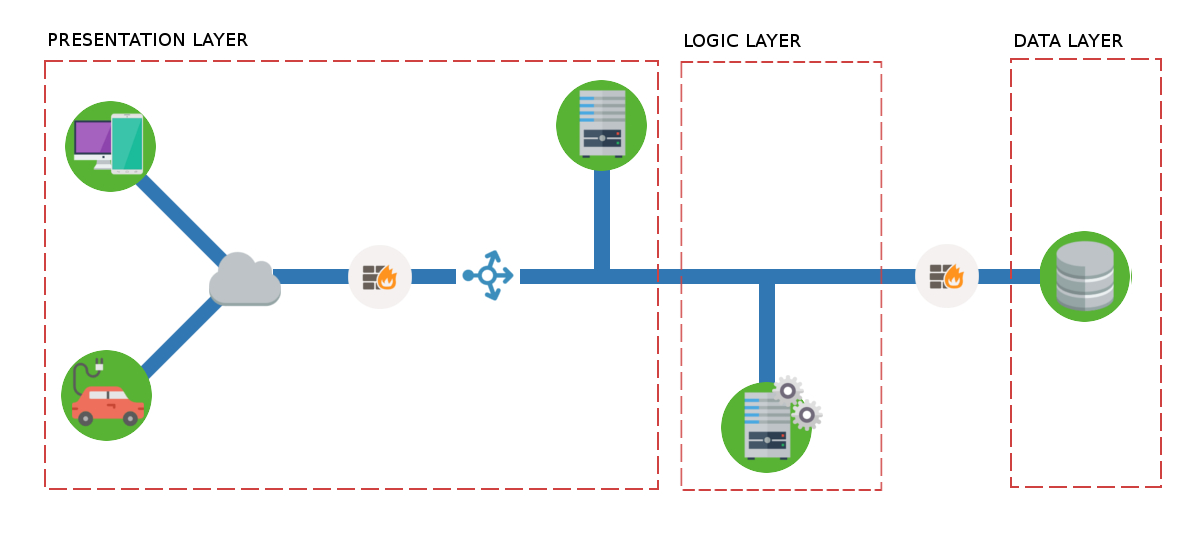
\includegraphics[width=350px]{../Datas/images/PEhla.jpg}
	}
		\caption{The system's high-level architecture}
		\label{fig:high-lev-arch}
\end{figure}


The general architecture of the system is based on the Client/Server paradigm. As depicted in Figure \ref{fig:high-lev-arch}, a suddivision in 3 layers, also called Distributed Representation is chosen:
	\begin{itemize}
		\item Presentation level: the level where information requested are presentend (i.e: rendered by means of a web browser or simply delivered to the final user).
		\item Application logic level: here the whole logic of the system take place (i.e: vehicles' availability control).
		\item Data level: where the datas used, created and modified by the application logic tier are stored.
	\end{itemize}

The elastic load balancer cloud computing patter is used and placed in front of the web servers and the application logic servers in order to increasethe availability of the system.
To mitigate security issues, firewalls are located between Application logic tier and Datas tier and in between of the public internet and the system's private network.
